\documentclass[a4paper]{article}
\usepackage[left=2.1cm, right=2.1cm, top=2.1cm]{geometry}
\usepackage{lipsum}
\usepackage{tikzpagenodes}
\usepackage{pgfplots}
\usepackage{tikz}
\usepackage{tikz-3dplot}
\usetikzlibrary{arrows,decorations.pathmorphing,backgrounds,positioning,fit,matrix}
\pgfplotsset{compat=1.8}
\usepackage{graphics} % for pdf, bitmapped graphics files
\usepackage{epsfig} % for postscript graphics files
\usepackage[colorlinks=true,citecolor=green]{hyperref}
\usepackage{cite}
\usepackage{amsmath,amssymb,amsfonts}
\usepackage{algorithmic}
\usepackage{graphicx}
\usepackage{url}
\usepackage{cite}
\usepackage{bm}
\usepackage{pbox}
\usepackage{siunitx,booktabs,etoolbox}
\usepackage{ulem}
\usepackage[framed,numbered,autolinebreaks,useliterate]{mcode}
\usepackage{filecontents}
%\usepackage{bigfoot} % to allow verbatim in footnote


\def\BibTeX{{\rm B\kern-.05em{\sc i\kern-.025em b}\kern-.08em
    T\kern-.1667em\lower.7ex\hbox{E}\kern-.125emX}}


\begin{document}

\title{Exercise on image stiching using IMU}
\author{xiahaa@space.dtu.dk}
\maketitle%%

In this exercise, you will work on using IMU of image stiching. IMU usually refers to Inertial Measurement Unit. 
\section{IMU}
If you search with Google or Alibaba, then probably you will find something with a similar name but with a prefix like $3$-axis, $6$-axis, and $9$-axis which corresponds to the sensors integrated inside the IMU. For example, if one IMU only contains $3$-axis gyroscope (for measuring angular velocity), then it will be called as $3$-axis IMU. If besides gyroscope, it also includes a $3$-axis accelerometer (for measuring acceleration) and will be called as $6$-axis IMU. 

High-end IMU is very accurate and expensive, which is often used in aeroplanes, fighters, missiles. Low-end IMU is very cheap and widely used in various products, like mobile-phones, action cameras, AR, etc.

In this exercise, we will only use the data provided by low-end IMU. The data is obtained from the ESE650 given at University of Pennsylvania\footnote{\url{https://upenn.box.com/v/ese650Proj2-train}}. Sensor fusion is needed in order to get accurate accurate information. Code has been provided to you for this part. The filter used here is the so-called complementary filter on Special Orthogonal Group ($\mathbb{SO}(3)$).
\begin{figure*}[!b]
	\centering
	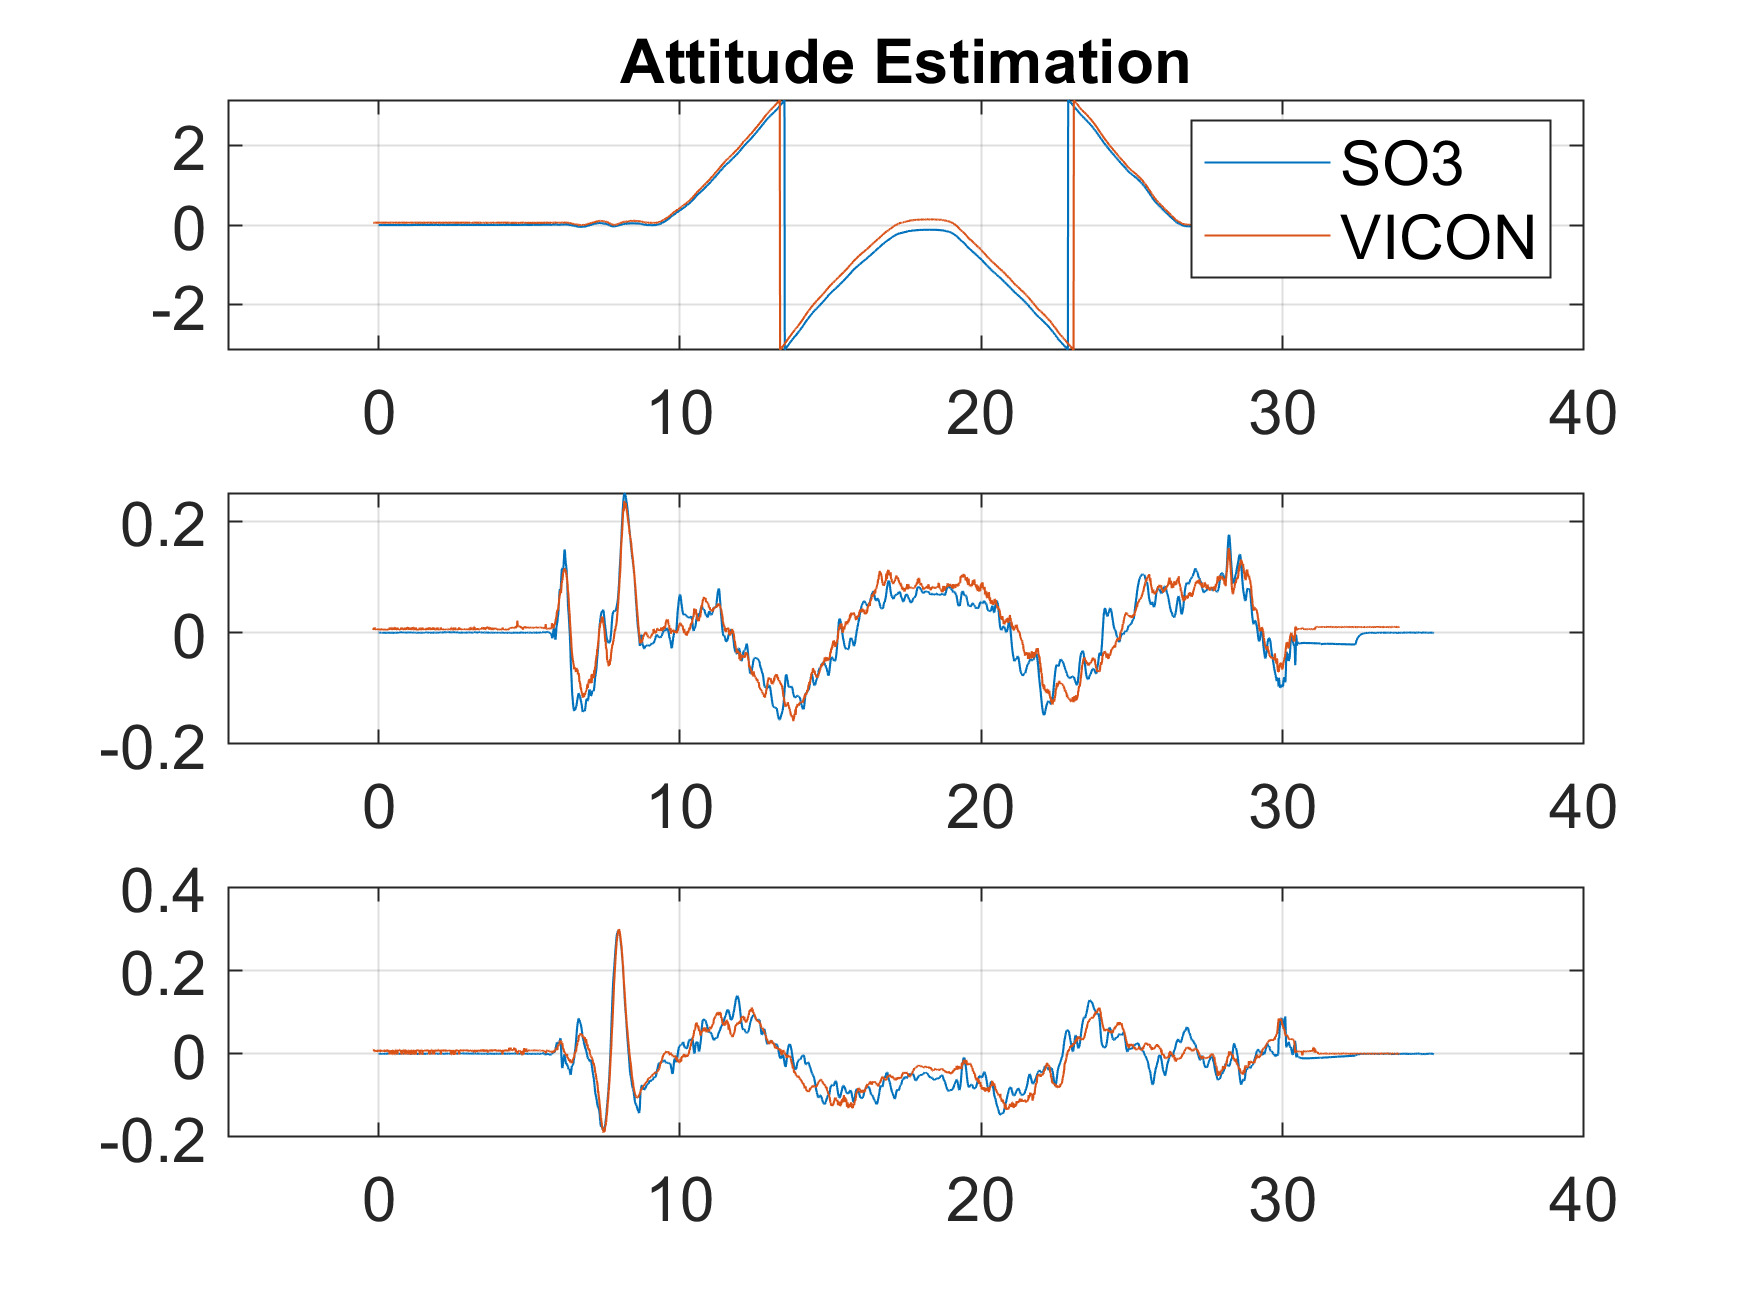
\includegraphics[scale=0.9]{figures/so3_1.png}
	\caption{Example of attitude estimation result.}
	\label{fig1}
\end{figure*}
An example of the sensor fusion result is shown in Figure~\ref{fig1}. VICON is a motion capturing system which can be used as the ground truth. As can be seen, the fusion algorithm is fairly good and the errors are quite small.

\section{IMU aided image stiching}
Since low-end IMU can only give us attitude information, the image stiching will be done using the cylindrical projection. Cylindrical projection is nothing but project each pixel into a cylindrical coordinate system. In order to accomplish this, you need to do as follows:
\begin{enumerate}
\item estimate the camera focus length $f$. A rough estimation of $f$ can be done as
\begin{align*}
f = \frac{0.5width}{tan(\frac{FOV}{2})}
\end{align*}
where $width$ means the image width, $FOV$ is the Field-Of-View (you can use $\frac{\pi}{3}$ here).
\item The cylindrical projection is shown in Figure~\ref{fig2}. So basically, you need to transform every pixel of the image to its corresponding point on cylindrical surface. This has to be done in several steps:
\begin{itemize}
\item move origin to principle point, so $(u,v)\to (u-c_u,v-c_v)$ (so point on the left (right) will have a negative (positive) x coordinate).
\item point in camera frame to point in IMU frame $\mathbf{p}_{imu}=\mathbf{R}_{cam}^{imu}\mathbf{p}_{cam}$, here $\mathbf{R}_{cam}^{imu}=\left[\begin{matrix}
0&0&1\\-1&0&0\\0&-1&0\\
\end{matrix}\right]$.
\item point in Cartesian frame to Cylindrical frame
\begin{align*}
r &= \sqrt(x^2+z^2) \\
x &= \frac{x}{r} \\
y &= \frac{y}{z}  \\
z &= \frac{z}{r}
\end{align*}
\item to point in initial global cylindrical frame $\mathbf{p}_{glb}=\mathbf{R}_{imu}^{glb}\mathbf{p}_{imu}$, here $\mathbf{R}_{imu}^{glb}$ is from sensor fusion algorithm.
\item to $\theta,h$ by $\theta=-atan2(z,x)$ and $h=-y$ (negative because the top left starts with $(1,1)$ in the image).
\item add $cu,cv$. $cu,cv$ is the center of the stiched image. For example, you can use $\frac{w}{2},\frac{h}{2}$ as the center.
\end{itemize}
Tips that can make this process faster: the first three steps are constant, so they only need to be done once.

\textbf{This may be complex for you. So if you have problem, just ask.}

\end{enumerate}
\begin{figure*}[!b]
	\centering
	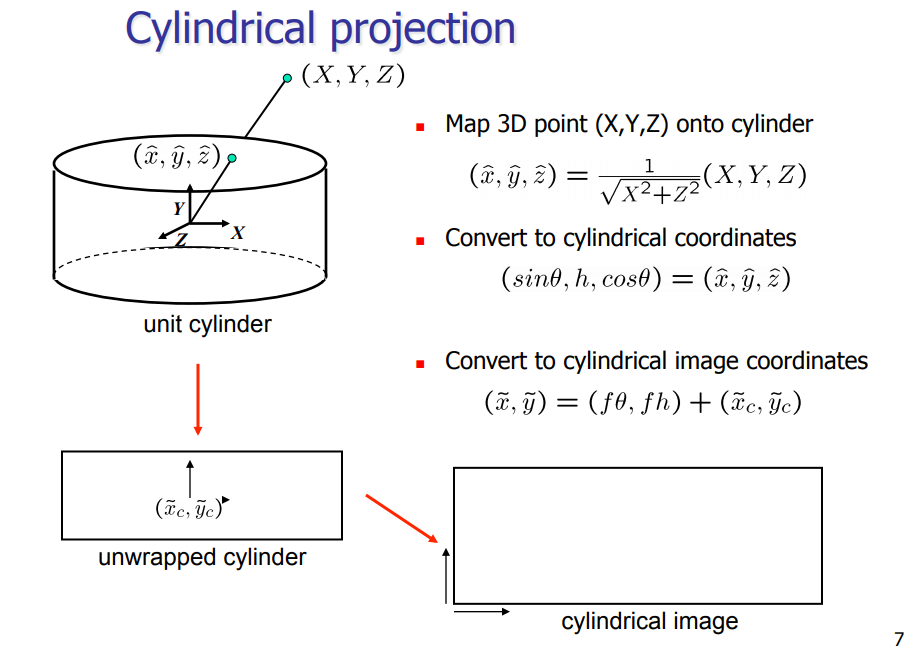
\includegraphics[scale=0.5]{figures/cylin_proj.png}
	\caption{Cylindrical projection, figure from \url{https://cs.gmu.edu/~kosecka/cs482/lect-panoramas.pdf}.}
	\label{fig2}
\end{figure*}

\end{document}